\subsection{Begriffserklärung Zwischensystem und Endsystem}

    Ein \textbf{Endsystem} oder Endgerät ist ein Computer oder ein anderes Peripheriegerät, an welchem keine weiteren Geräte angeschlossen sind. \\
    Beispiele für Endsysteme sind:
    \begin{itemize}
        \item Drucker
        \item Geldautomat
        \item Surfstation
        \item Lautsprecher
        \item Kamera
    \end{itemize}
    \
    Außerdem muss es \textbf{Zwischensysteme} geben, die gesendete Datenpakete an die richtige Adresse weiterleiten. \\
    Solche Zwischensysteme sind Switches, Bridges und Router. 


\subsection{Nutzen der Protokollschichten des Osi-Modells}

    Das OSI Modell ist ein Modell, welches die Ebenen die ein Netzwerk ausmachen beschreibt.

    \renewcommand{\tabcolsep}{1pt}
\begin{longtable}{@{}p{0.3\textwidth}@{\hspace{3em}}p{0.6\textwidth}}
    \\\hline
    \makecell[l]{Bitübertragungsschicht \\ (Physical Layer)}
        & 
        \begin{itemize}
            \item elektrische / physische Übertragung der Daten 
        \end{itemize}
        
    \\\hline

    \makecell[l]{Sicherungsschicht \\ (Data Link Layer)}
        &
        \begin{itemize}
            \item alle Vorkehrungen, die dafür sorgen, dass aus der physikalischen Übertragung ein verlässlicher Datenfluss wird
        
        \end{itemize}
    \\\hline
    
    \makecell[l]{Vermittlungsschicht \\ (Network Layer)}
        &
        \begin{itemize}
            \item Komponenten und Protokolle, die an der Verbindung zwischen Rechnern beteiligt sind - das sogenannte Routing - Weiterleiten von Daten in andere logische und oder physikalisch inkompatible Netzwerke
        \end{itemize}
    \\\hline
    
    \makecell[l]{Transportschicht \\ (Transport Layer)}
        &
        \begin{itemize}
            \item verbindungsorientierte Protokolle wie TCP und verbindungslose Protokolle wie UDP
            \item ein wichtiger Aspekt dieser Schicht ist Multiplexing - Anbindung der Datenpakete an konkrete Prozesse auf den kommunizierenden Rechnern 
            \item Segmentierung des Datenstroms und Datenstauvermeidung
        \end{itemize}
    \\\hline

    \makecell[l]{Kommunikationssteuerungsschicht \\ (Session Layer)}
        &
        \begin{itemize}
            \item sichert Kommunikation zwischen kooperierenden Anwendungen oder Prozessen auf verschiedenen Rechnern
            \item organisiert und synchronisiert Datenaustausch
        \end{itemize}
    \\\hline

    \makecell[l]{Darstellungsschicht \\ (Presentation Layer)}
        &
        \begin{itemize}
            \item Konvertierung und Übertragung von Datenformaten, Datensätzen, Zeichensätzen, grafische Anweisungen und Dateidienste
            \item systemabhängige Darstellung von Daten
            \item Datenkompression, Verschlüsselung
            \item stellt sicher, dass Daten die von der Anwendungsschicht des einen Systems gesendet werden von der Anwendungsschicht eines anderen Systems gelesen werden können
        \end{itemize}
    \\\hline

    \makecell[l]{Anwendungsschicht \\ (Application Layer)}
        &
        \begin{itemize}
            \item unmittelbare Kommunikation zwischen Benutzeroberflächen der Anwendungsprogramme
            \item Das Anwendungsprogramm selbst zählt nicht dazu
        \end{itemize}
    \\\hline

    
\end{longtable}


    \begin{figure}[H]
        \centering
        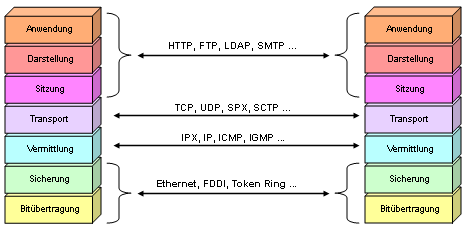
\includegraphics[width=0.7\textwidth]{vorbereitung/Osi.png}
        \source{Osi Modell}{https://www.der-wirtschaftsingenieur.de/bilder/it/OSI-Modell3.PNG}{3.1.2020 14:30}
    \end{figure}
    \
    \textbf{Repeater}
    \\
    Ein Repeater verstärkt ganz simpel die elektronischen Signale und nutzt deswegen nur die 1. Schicht des OSI-Models. Der in der Abbildung unterhalb veranschaulichte HUB (Multi-Port-Repeater) sendet ein von PC0 gesendetes Paket an alle anderen PC’s weiter, da er keine Möglichkeit hat, an ein bestimmtes Gerät zu senden, da er keine MAC-Adressen speichert. Er teilt keine Broadcastdomäne.\\

    \begin{figure}[H]
        \centering
        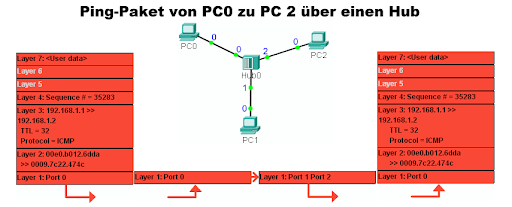
\includegraphics[width=0.7\textwidth]{vorbereitung/ping_hub.png}
        \source{Ping über einen Hub}{https://www.tinohempel.de/info/info/netze/osi.htm}{8.1.2020 13:00}
    \end{figure}
    \
    \textbf{Bridge}
    \\
    Eine Bridge verbindet mehrere über Kabel verbundene Netzwerke / PCs miteinander, sodass sie ein einzelnes Netz repräsentieren. In Bezug auf das OSI Modell werden über die erste Schicht Signale versandt und über die zweite Schicht werden die Signale einem Zielort via einer Link-Layer-Address zugeordnet. In der folgenden Abbildung sieht man einen Switch (Multi-Port-Bridge), welcher die von PC0 gesendeten Pakete anhand der MAC-Adresse, aus dem entsprechenden Port, an PC2 weiterleitet. \\

    \begin{figure}[H]
        \centering
        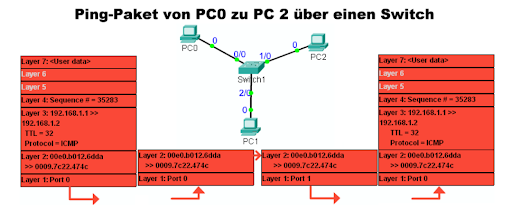
\includegraphics[width=0.7\textwidth]{vorbereitung/ping_bridge.png}
        \source{Ping über einen Switch}{https://www.tinohempel.de/info/info/netze/osi.htm}{8.1.2020 13:00}
    \end{figure}
    \
    \textbf{Router}
    \\
    Ein Router verbindet mehrere Netzwerke miteinander. Anhand von Routing-Tabellen (statisch oder dynamisch) leitet er die Datenpakete in die entsprechende Netze oder über ein Default-Gateway weiter. Die Routing-Entscheidungen geschehen aufgrund von IP-Adressen (OSI-Layer 3) und ggf. weiteren Parametern z.B. anhand der Pfadkosten beim OSPF-Protokoll. PC0 sendet das Datenpaket an Router1 mit seiner IP-Adresse als Quelladresse und der Zieladresse (PC2). Der Router kennt das Zielnetz, da es direkt angeschlossen ist und sendet es an PC2 weiter.\\

    \begin{figure}[H]
        \centering
        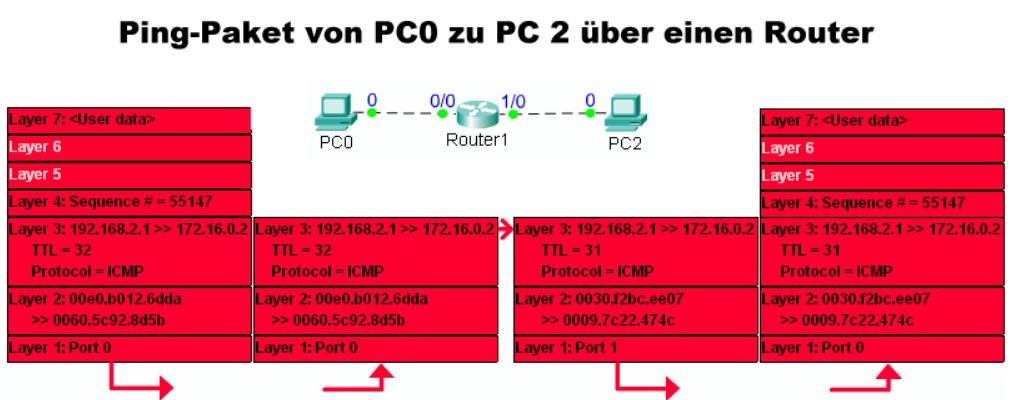
\includegraphics[width=0.7\textwidth]{vorbereitung/ping_router.png}
        \source{Ping über einen Router}{https://www.tinohempel.de/info/info/netze/osi.htm}{8.1.2020 13:00}
    \end{figure}
    \
    \textbf{Gateway}
    \\
    Ein Gateway ist ein computer-ähnliches Gerät, welches eine Kommunikation zwischen zwei oder mehr unterschiedlichen Systemen herstellt. Ein Gateway kann Software oder Hardware sein. Um mit verschiedenen Arten von Netzwerken zu kommunizieren, muss der Netzwerk Gateway auf mehreren Schichten des OSI Modells operieren, unter Umständen auch auf allen 7, da er zum Beispiel Sessions erstellen und verwalten muss, Daten entschlüsseln und unterschiedliche physikalische und logische Adressen übersetzen muss. Wegen der vielen Aufgaben die ein Gateway gleichzeitig erledigen muss ist er um einiges langsamer, als die anderen oben genannten Geräte. Der Gateway, der in der Aufgabenstellung dargestellt wird greift auf alle 7 Layer zu und muss deswegen eine Software auf einem Computer sein, auf die ein Benutzer via einer Oberfläche zugreifen kann.\\

\subsection{Einordnung von Switch und Layer-3-Switch in Abbildung}

    \textbf{Switch}
    \\
    Ein Layer-2-Switch arbeitet mit Data-Link Layer-Adressen (MAC). Er benutzt also nur die Bitü- bertragungsschicht und die Sicherungsschicht. Er sendet die Daten weiter an einen fest ange- gebenen Punkt anhand der MAC-Adressen. \\
    Er ist als Äquivalent zur Bridge zu sehen. Denn er ist im Prinzip eine Multi-Port-Bridge und im Gegensatz zum HUB, erzeugt er keinen unnötigen Traffic, da nur an ein bestimmtes Ziel und nicht an alle gesendet wird (durch MAC-Adressen-Tabelle).\\
    \\
    \textbf{Layer-3-Switch}
    \\
    Ein Layer-3-Switch ist ein Switch, welcher um die Routing-Funktionen erweitert wurde und sonst alle Funktionen von einem Layer-2-Switch beibehält. Deshalb ist er mit dem Router aus Abbildung 1 gleichzusetzen. Durch die Erweiterung auf Layer 3 unterstützen diese Switches auch Inter-VLAN-Routings. Erweiterte Funktionen, wie NAT, IPSec oder Firewall-Filtering werden allerdings nicht unterstützt.



\subsection{Zweck und Header-Aufbau von ICMP, Nutzung des Protokolls in der Konsole unterschiedlicher Betriebssysteme}
    Das ICMP (Internet Control Message Protocol) tauscht Informations- und Fehlermeldungen über IPv4 in Rechnernetzen aus. Das Äquivalent in IPv6 heißt ICMPv6.
    Für jeden Rechner und Router ist es Standard, dass sie ICMP verstehen.\\
    ICMP Pakete dienen dazu Diagnose Informationen zurück an die Quelle zu senden, wenn der Router Pakete verwirft. Beispielsweise, wenn das Ziel nicht erreichbar ist oder die TTL abgelaufen ist.
    So wird zum Beispiel mit dem Befehl “ping” ein Test Datenpaket über das ICMP Protokoll gesendet.
    \begin{itemize}
        \item Zweck, Headeraufbau
        \item Nutzung in der Konsole unterschiedlicher Betriebssysteme
    \end{itemize}

    Der Befehl ping ist unter den meisten Betriebssystemen wie Windows, Linux (und anderen Unixartigen), Unix oder macOS, aber auch als Analysetool auf Geräten wie Routern nutzbar. Die Ausführung des Befehls und somit die Aussendung der ICMP Pakete unterscheiden sich jedoch je nach Betriebssystem, so sendet Windows eine begrenzte Anzahl an Paketen während Linux eine unbegrenzte Anzahl sendet und nur manuell abgebrochen werden kann.

    \begin{figure}[H]
        \centering
        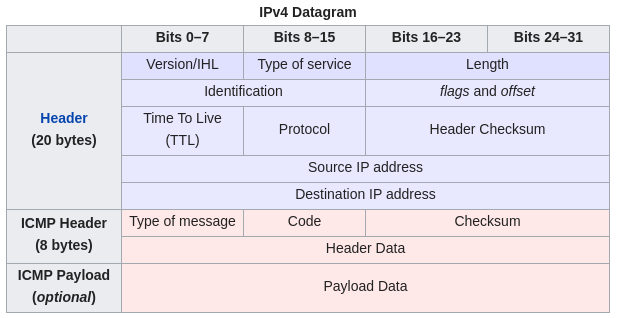
\includegraphics[width=0.5\textwidth]{vorbereitung/IPv4_Datagramm.png}
        \source{IMCP Aufbau IPv4}{https://en.wikipedia.org/wiki/Ping\_\(networking\_utility\)\#ICMP\_packet}{2.1.2020 15:00}
    \end{figure}
    \begin{figure}[H]
        \centering
        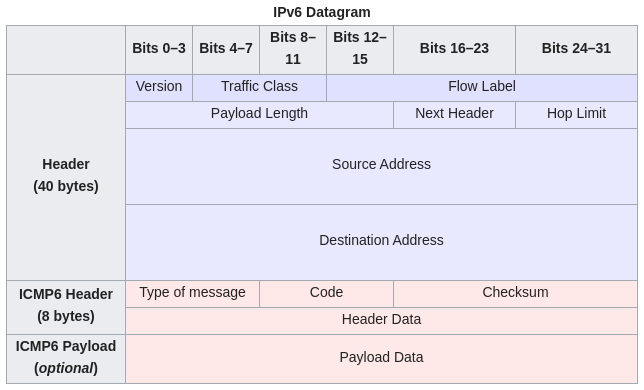
\includegraphics[width=0.5\textwidth]{vorbereitung/IPv6_Datagramm.png}
        \source{IMCP Aufbau IPv6}{https://en.wikipedia.org/wiki/Ping\_\(networking\_utility\)\#ICMP\_packet}{2.1.2020 15:00}
    \end{figure}




\subsection{Peer-2-Peer Netzwerk entsprechend DFÜ-Modell}

    DDE bezeichnet die Datenendeinrichtung und stellt den Sender oder den Empfänger dar. Sie kontrolliert und steuert die Datenfernübertragung.\\
    DÜE bezeichnet die Datenübertragungseinrichtung. Sie ist die Verbindung zwischen den DDE’s und dem Netzwerk und wandelt die Daten in eine geeignete Form für die Übertragung um.\\
    Zwischen DDE und DÜE befindet sich eine serielle Schnittstelle (V.24, RS232), ein USB Kabel oder eine Funkverbindung wie Bluetooth.\\

    \begin{figure}[H]
        \centering
        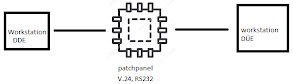
\includegraphics[width=0.5\textwidth]{vorbereitung/DFUE.png}
        \source{DFÜ Modell}{eigene Zusammenstellung}{}
    \end{figure}
\subsection{Skizze des Protokollstapels}

    \begin{figure}[H]
        \centering
        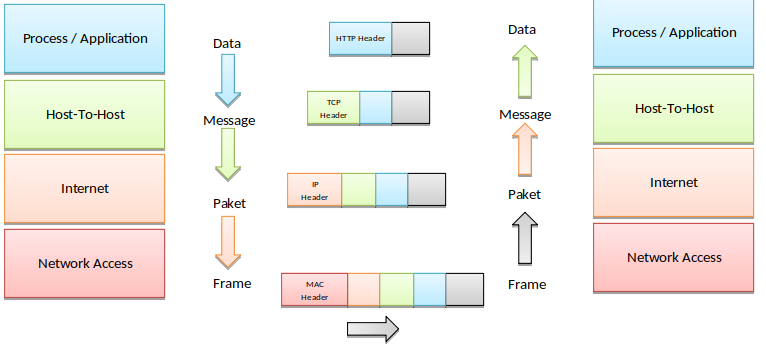
\includegraphics[width=0.5\textwidth]{vorbereitung/Protokollstapel.png}
        \source{Skizze eines Protokollstapels eines HTTP Requests}{eigene Zusammenstellung}{}
    \end{figure}
\pagebreak
\subsection{Headerstruktur für HTTP, TCP, IPv4, IPv6 und Ethernet}

    \textbf{Http Response Header}
    \\
    Übergeben zusätzliche Informationen über die Antwort, die nicht in die Status Line passen. Sie Enthalten Informationen über den Server und weitere Zugänge zu der Quelle. Diese sind durch die Request-URI gekennzeichnet.\\

    \begin{figure}[H]
        \centering
        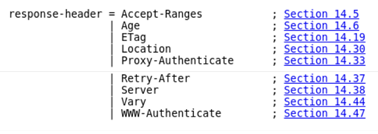
\includegraphics[width=0.5\textwidth]{vorbereitung/http_response_header.png}
        \source{HTTP Response Header}{http://www.coder-welten.de/glossar/request-und-response-18.html}{07.01.2020 15:00}
    \end{figure}

    \textbf{HTTP Request Header}
    \\
    Geben zusätzliche Informationen über den Request mit, wie über den Client selbst, zum Server. \\
    \begin{figure}[H]
        \centering
        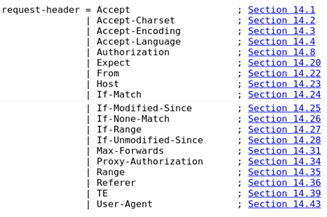
\includegraphics[width=0.5\textwidth]{vorbereitung/http_request_header.png}
        \source{HTTP Request Header}{http://www.coder-welten.de/glossar/request-und-response-18.html}{07.01.2020 15:00}
    \end{figure}

    \textbf{TCP Header}
    \\
    Dieser Header enthält die zur Kommunikation erforderlichen Daten und Dateiformat-beschreibende Informationen. Normalerweise sind TCP Header 20 Bytes lang, können aber mit den kaum genutzen Optionen erweitert werden.\\

    \begin{figure}[H]
        \centering
        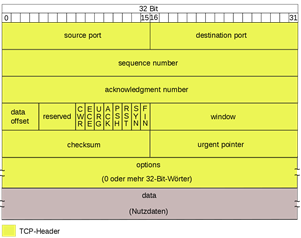
\includegraphics[width=0.5\textwidth]{vorbereitung/TCP_Header.png}
        \source{TCP Header}{https://upload.wikimedia.org/wikipedia/commons/thumb/f/fd/TCP\_Header.svg/1024px-TCP\_Header.svg.png}{2.1.2020 14:00}
    \end{figure}

    \textbf{IPv4 Header}
    \\
    Die Länge von IPv4 Header ist normalerweise 20 Bytes, kann aber mit bestimmten Optionen auf bis 60 Bytes erweitert werden.\\

    \begin{figure}[H]
        \centering
        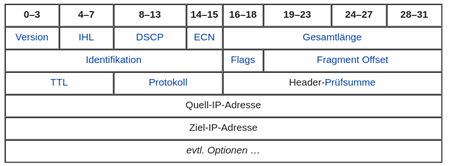
\includegraphics[width=0.5\textwidth]{vorbereitung/IPv4_Header.png}
        \source{IPv4 Header}{https://de.wikipedia.org/wiki/IPv4\#Header-Format}{2.1.2020 14:30}
    \end{figure}

    \textbf{IPv6 Header}
    \\
    Hat eine feste Länge von 40 Bytes. Optionale selten genutzte Daten können in Extension Headern zwischen Header und Payload gesendet werden.\\

    \begin{figure}[H]
        \centering
        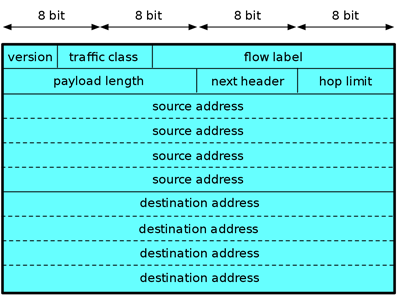
\includegraphics[width=0.5\textwidth]{vorbereitung/IPv6_Header.png}
        \source{IPv6 Header}{https://upload.wikimedia.org/wikipedia/commons/thumb/c/cd/IPv6\_Header.svg/1280px-IPv6\_Header.svg.png}{2.1.2020 14:45}
    \end{figure}
    \pagebreak
    \textbf{Ethernet}
    \\
    Enthält die Zieladresse (6 Bytes), Quell-MAC-Adresse (6 Bytes), das EtherType field (2 Bytes) und optional einen IEEE 802.1Q tag oder einen IEEE 802.1ad tag (4 Bytes).

\subsection{Analyse von Anweisungen für das Protokoll IPv6}
    \renewcommand{\tabcolsep}{1pt}
\begin{xltabular}{\textwidth}{@{}p{0.4\textwidth}@{\hspace{3em}}p{0.6\textwidth}@{}}
    \\\hline
    \makecell[l]{netsh interface ipv6 show interfaces \\ (füher ipv6 if)}
        &
    \makecell[l]{
        Pingt das angegebene Interface an und gibt dabei die link-layer-adress, die ipv6 Adressen die zu dem Interface gehören und das aktuelle MTU und die maximale Anzahl der MTU’s die das Interface unterstützen kann.\\
        Interface 1 ist ein Pseudo-Interface.\\
        zeigt an:\\
            \textbf{Index} - Bereichskennung \\
            \textbf{Met} - gibt die Pfadkosten an, je niedriger, desto besser, kann wenn es mehrere Routen gibt dazu verwendet werden zu entscheiden, welche Route verwendet wird\\
            \textbf{MTU} - maximale Anzahl an MTU’s die das Interface unterstützt\\
            \textbf{state} - status des Interfaces, ist Interface enabled Oder disabled\\
            \textbf{name} - Name des Interfaces
    }
    \\\hline
    ping -6 ::1
    &
    Pingt den localhost an. Das heißt es wird ein ICMP-Paket mit einem TTL Wert von 128 gesendet und kommt vom localhost wieder zurück.
    \\\hline
    ping -6 Adresse\%Bereichskennung
    &
    Pingt die Adresse über das in der Bereichskennung angegebene Interface an. Zum Beispiel wenn man die Adresse fe80::1\%SCHNITTSTELLE einen ping heraus sendet, wird ein ICMP Paket an die Link-Local-Adress fe80::1 über die Schnittstelle “SCHNITTSTELLE” an.
    \\\hline
    netsh interface ipv6 show route
    &
    \makecell[l]{
        Pingt jeden Hop bis zum Host an und verfolgt dabei die Route.\\
        Dabei werden ICMP-Pakete mit immer höher werdendem TTL-Wert ausgesandt, die dann nacheinander von den beteiligten Routern bearbeitet werden. Der höchste TTL-Wert entspricht dann dem des Hosts.\\
        Die Ausgabe zeigt dann die Hops bis zum Ziel an.\\
        Angezeigt werden:\\
            - Der wie vielte Hop wurde bewältigt\\
            - die Zeit die gebraucht wurde um den Hop zu bewältigen\\
            - die IP des Hops und die Benennung
    }

\end{xltabular}